Wireless Sensor Networks are being used more and more in almost every field imaginable in order to collect and improve our life, fileds like home automation, agriculture, military, space exploration etc. In order to collect the data, gateway platforms \cite{hill2004platforms,da2011design,da2011design2} are required and most of them are stationary bulky devices or PCs connected to one of the wireless nodes that serve as a base-station. We aim to show in this paper that there exists a solution for a truly mobile gateway design that can be used either for collecting data or for debuging large wireless network infrastructures.

We have conected to an AR Parrot Drone 2.0 our SparrowDongle, a USB stick featuring two microcontrollers that can connect to 2.4GHz Zigbee nodes or to our own node design Sparrowv3.2. We will show an overview of the system
architecture in Chapter \ref{chap:arch}, the hardware and software
implementation in Chapter \ref{chap:impl} and results of using the gateway in
Chapter \ref{chap:results}. 

\begin{figure}[ht] \centering
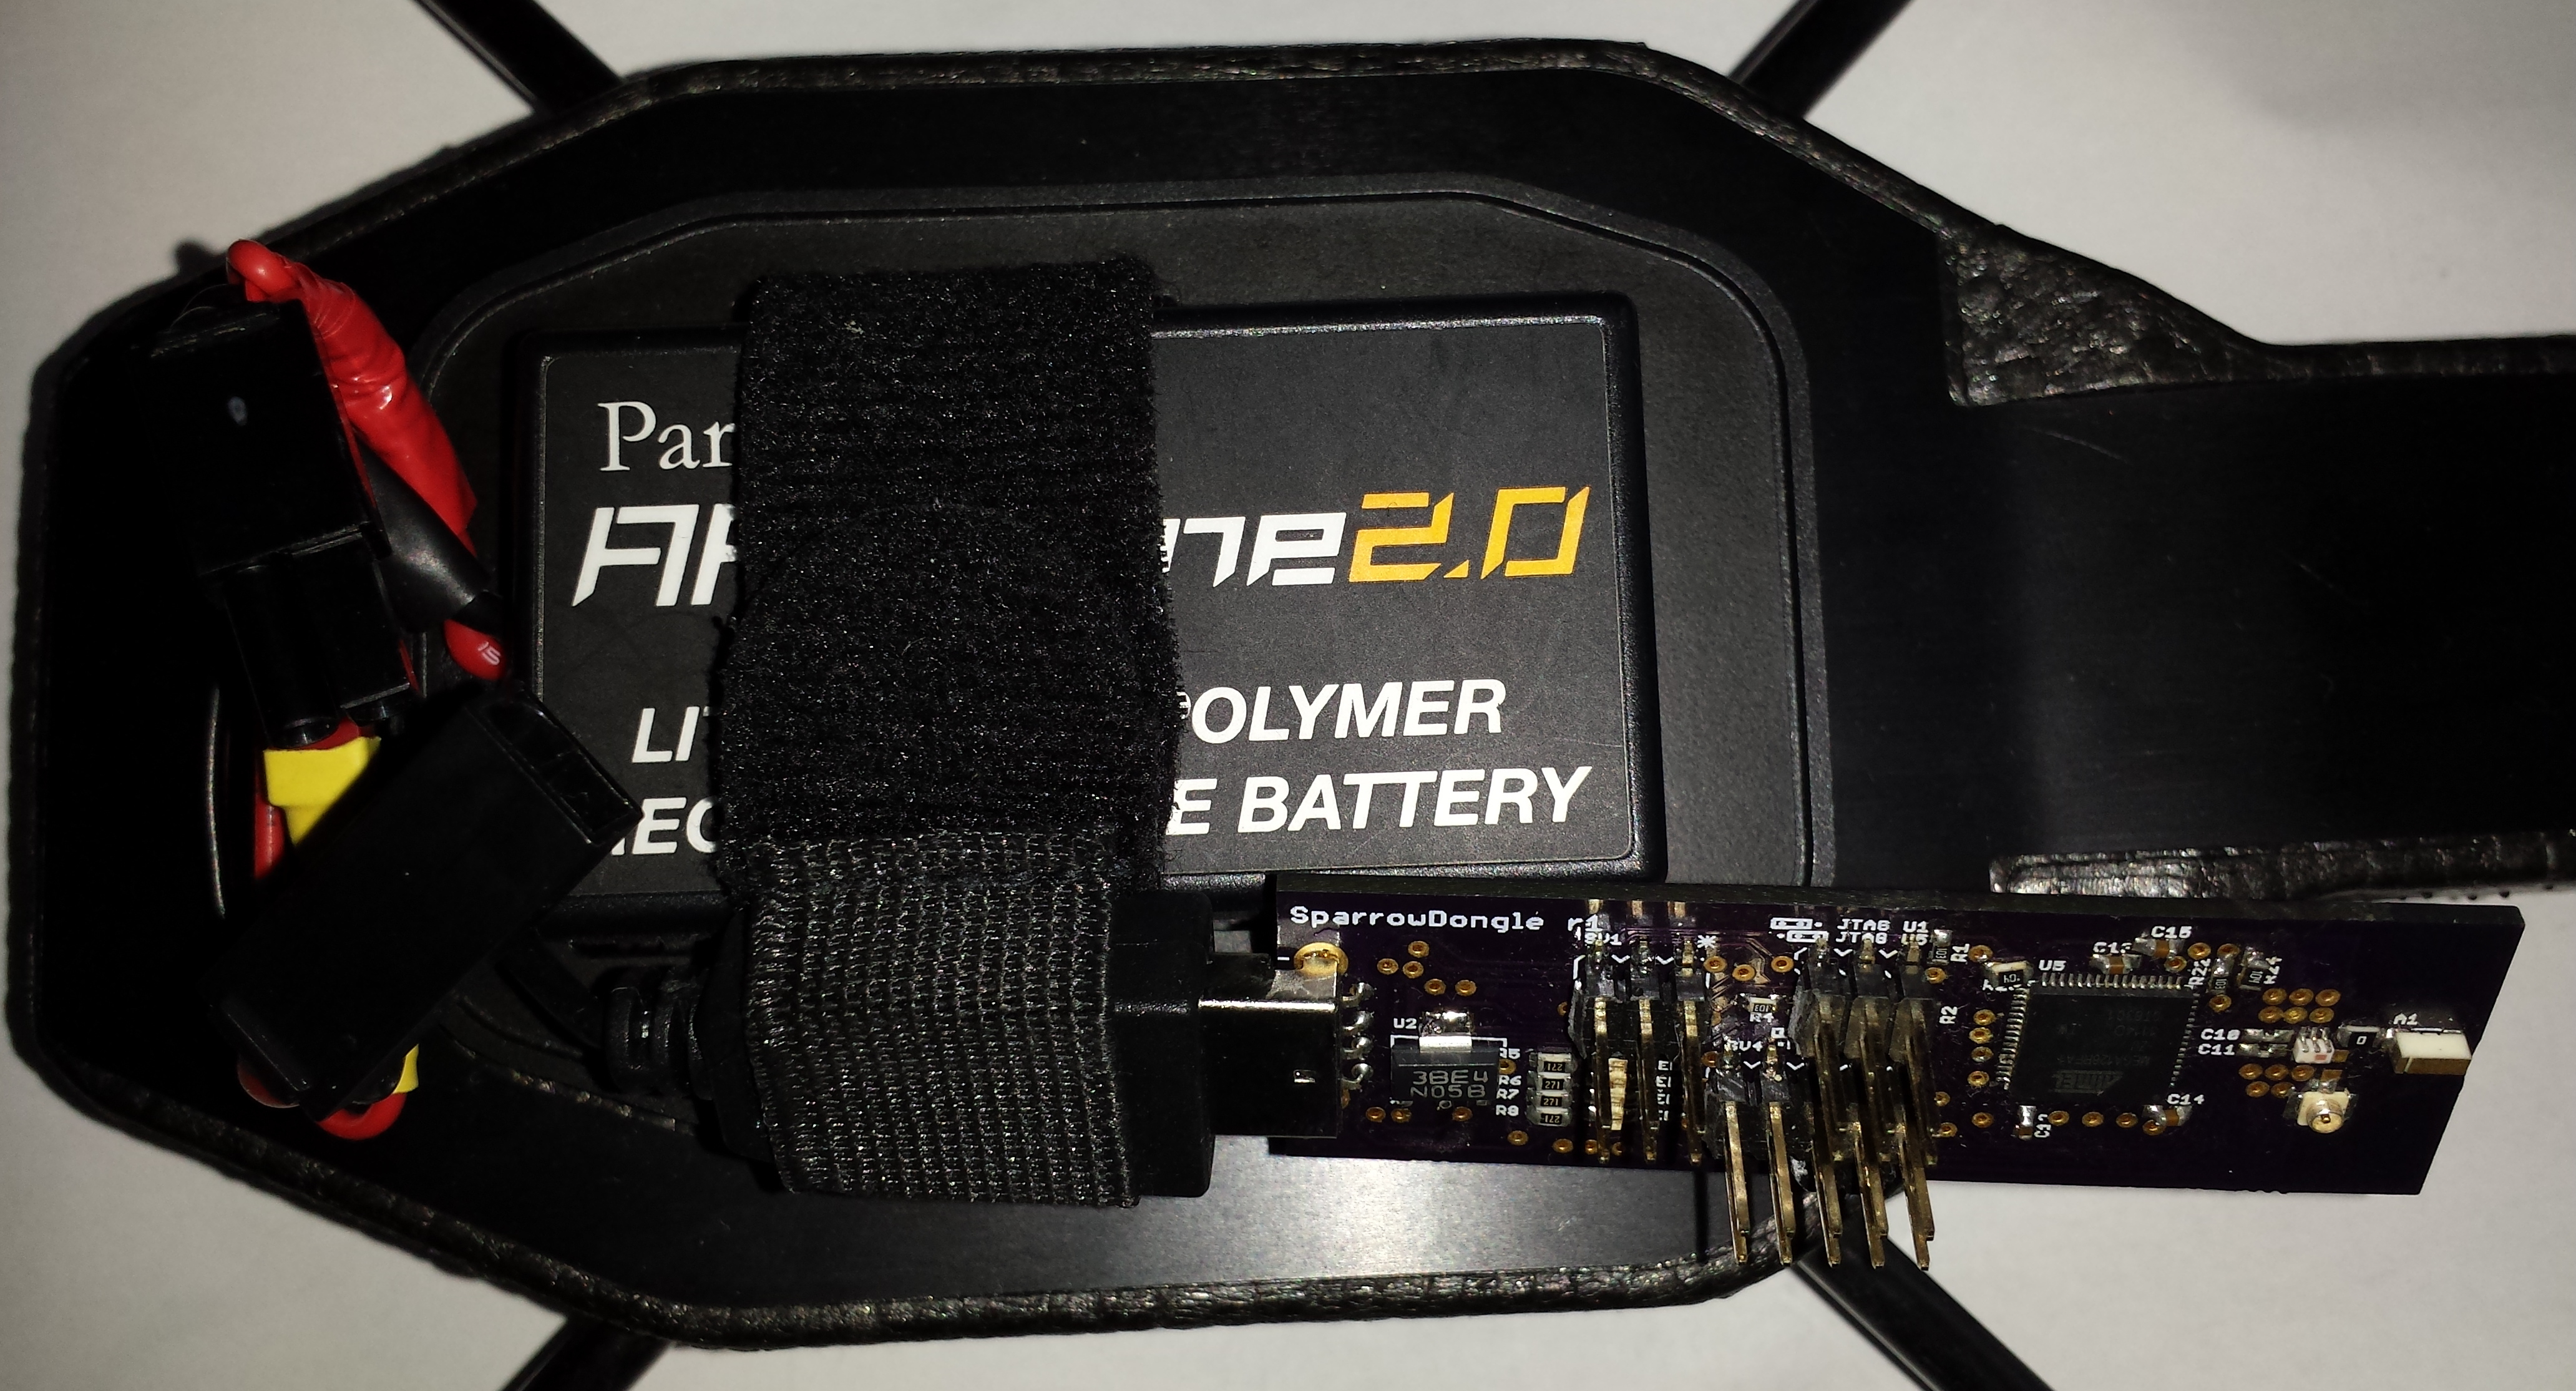
\includegraphics[width=0.45\textwidth]{img/dronedongle.jpg} \caption{SparrowDongle connected to AR Parrot Drone 2.0 } \end{figure}


